
\section{Introduction}

The aim of the development of NODUS is to offer a new solution to the problems
posed by the flows of goods on a multi-modal transportation network.  In that
respect, this chapter, which is a short theoretic repetition of the concepts on
which the development of transportation networks is based, will be essentially
limited to the most important modal-choice and assignment models, so that these
can be compared to the models that have been applied to NODUS.  However, since
it is necessary to have matrixes of origins-destinations (O-D) in order to apply
the modal choice and the assignment, some generation and distribution methods
will also be dealt with in this chapter, as they can proof useful during the
practical applications\footnote{Although these matrixes are often treated as
external data.} of NODUS.


But before passing on to the different points mentioned above, some general
considerations on cost functions and on the behaviour of the different actors in
a transportation system in relation to the demand for transportation, are
certainly relevant here, since the (clear) definition of these functions and the
understanding of the role of the different actors are the key to the succes of a
model.



\subsection{General considerations on cost functions}

The notion of ''cost function'' will often be used in the different chapters
that constitute this methodological note.  These functions, however, are used in
contexts that may differ greatly, and, moreover, they do not always refer to the
same realities.  Furthermore, their (non) linearity will often be discussed.  In
order to adequately clarify these concepts, the different types of cost used
will be briefly dealt with.

First of all there are the ''cost functions linked to the links of a network''.
These are the costs \footnote{To avoid complicating things at this stage, the
term "cost" will be used for all financial charges.  It may concern, for
instance, a cost such as the wage of the driver when he uses his lorry.} borne
by a user who makes use of that segment of the network during a trip. The total
cost of transportation will often be considered to be proportional to the
distance covered and/or the quantity transported. Obviously, whenever there are
fixed costs, the average cost of transportation will not be linear. (See figure
\ref{f2_1}).

\begin{figure}[htbp]
\centerline{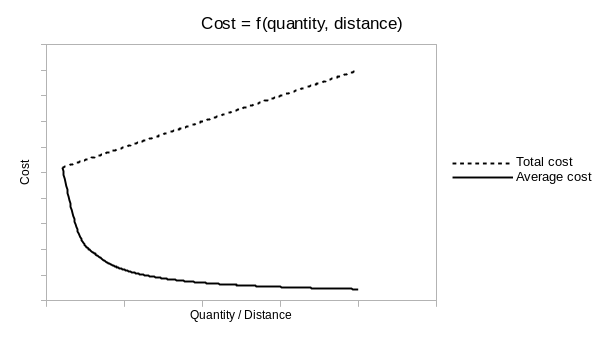
\includegraphics[width=12cm]{f2_1.png}}
\caption{\label{f2_1} Relation between quantity/distance and cost}
\end{figure}

However, the total costs on the links are not always proportional to the
quantity transported.  The costs of handling the goods, for instance, are not
proportional to the quantity of goods that are to be loaded and unloaded.


From the moment when congestion will have to be taken into account, the flow has
to be introduced (total quantity transported on a certain link) as a variable of
the cost function.  Thus the total cost of transportation expands exponentially
in proportion to that flow, as is illustrated in figure \ref{f2_2}.

\begin{figure}[htbp]
\centerline{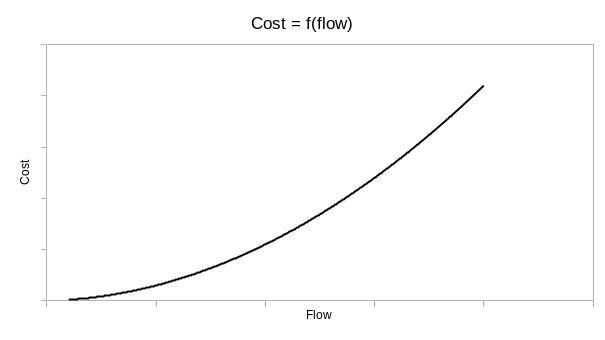
\includegraphics[width=12cm]{f2_2.png}}
\caption{\label{f2_2} Relation between flow and cost}
\end{figure}

The total cost on the transportation system remains to be considered.
Although there are several assignment methods on a network, they all have in
common that they minimize an objective function.  These objective functions can
also take different forms.  From a social viewpoint, it is important to minimize
the total cost of transportation on the system.  From the viewpoint of the user,
however, it is important to minimize the average cost of the trip.

Generally speaking, when the cost functions are proportional to the quantities,
and when congestion does not have to be taken into account, so that it is always
possible to assign the transportations by choosing the solution (choice of a
mode, a means or a route) with the lowest cost by applying an efficient
shortest-path algorithm, there is, properly speaking, no objective function as
long as there is discontinuity between the different possible solutions. But if
the costs of the different convex combinations of the solutions for the
assignment of the quantities are distinguished, the obtained cost function will
be a linear function since all the cost functions on the different links are
proportional to the quantities transported on those particular links.

However, when non-linear (convex) cost functions are used on the links, which
has to be the case for the models that take the level of congestion on a network
into consideration, the solutions will generally not be of the "all or
nothing"-type, but there will be a repartition of the quantities between the
different available modes, means and routes. The set of those possible solutions
constitutes a continuous convex function of the total cost resulting from the
addition of the different convex functions.

Several concepts relating to costs have to be taken into consideration, and for
this reason, all through this text, it will be clearly indicated what the costs
used refer to.


\subsection{The behaviour of the actors on a transportation system}

Traditionally, the actors that are taken into consideration are the producers of
goods (that play the role of shippers), the consumers and the carriers. The
producers and the consumers are not situated at the same location.  The analysis
of the mechanisms that control the links between those different actors is the
reason for which transportation economics exists and for which computer programs
such as NODUS have been developed these recent years.

The shippers are economic actors that decide to assign and to distribute a
certain flow of goods between an origin and a certain number of destinations.
The carriers represent in reality a set of different entities that are implied
in the decision of transportation.  This set covers for instance the departments
''shipments'', ''distribution'' or ''deliveries'' of the firms.  The decision of
transportation may be very intricate, but 'the only motivation that leads to
transport is an economic reason', as has been well explained by Roberts
\footnote{Roberts, P.O., 1976, ''Forecasting Freight Flows Using a Disaggregated
Freight Demand Model'', CTS Report 76-1, Center for Transportation Studies,
MIT.}.  Thus the decision of the carrier depends upon the fluctuations of supply
and demand, and of the prices on the market.

When the shipper decides to transport goods, he chooses a carrier to effect the
transportation.  In transportation economics, the carrier is always looked upon
as an economic agent that produces a service (transportation) while trying to
maximise his profit.

The relationship between the shippers and the carriers is compared to the
relationship between a consumer and a producer of services.  By his decision to
confide a shipment to a carrier, the shipper creates a demand for the output
produced by that carrier.  The carrier, on the other hand, will ask a certain
price for effecting the transportation task and will thus create a certain level
of service.


If the role played by the State is added to this, the existing relationships
between the different actors can be represented as shown in figure \ref{f2_3}:

\begin{figure}[htbp]
\centerline{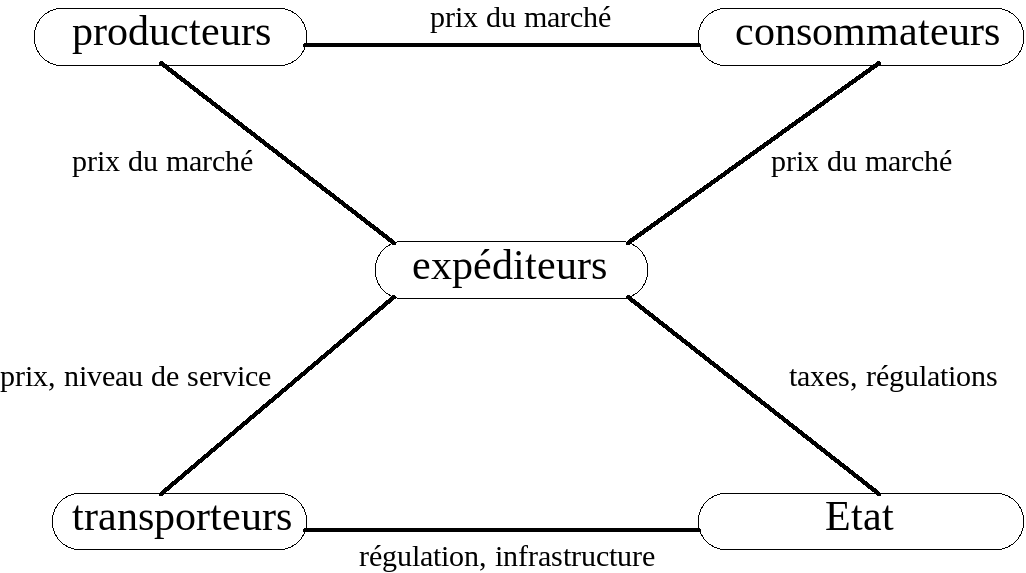
\includegraphics[width=10cm]{f2_3.png}}
\caption{\label{f2_3} The actors in a transport system}
\end{figure}



Nevertheless, it remains clear that all these interactions can only exist if
there is a demand for transportation.  That demand depends upon certain
explanatory factors among which :
\begin{itemize}

\item The price of the service of transportation : similar to the demand for
whatever product, the demand for transportation is in principle a decreasing
function of the price of transportation.

\item The price of the other modes of transportation : whereas certain categories
of goods are (almost) exclusively transported by one mode of transportation,
certain other categories qualify for several modes.  A price variation of one
mode of transportation can as a result influence the demand for another mode.

\item The price of the complementary goods : transportation can be considered
as a part of a production process.  A classical example is the
electric energy production of a power plant that has its coals or
fuel supplied by barges or by trucks.  It is clear that the demand for
transportation is a direct function of the level of energy production.

\item The duration : transportation is a particular product since the
user is "implied" in the production of the service of transport operation by the time
it takes for the goods to be moved.  The duration of the transportation plays a
highly important role for the demand for transportation and for the modal
choice.  The demand for transportation is inversely related to the amount of
time needed for the transport cycle.  The time-elasticity is therefore negative.
The demand for transportation is also influenced by the speed, but speed is
rather an element determining the duration of the transportation than a
supplementary explanatory factor.

\item The freedom of choice : the shippers are highly sensible to this factor,
which partly explains the succes of road transportation.

\item The capacity : the correspondence between the characteristics of the goods that
are to be transported (volume, weight) and those of the mode of transportation
often determine the modal choice.

\item The security and the observance of the time schedules: the transportations of
goods are influenced by the inherent risks (although the perception of that risk is
often subjective) and by the time constraints that are imposed .

\end{itemize}

\section{Generation and distribution techniques}

This section focusses on some basic techniques concerning the generation and the
distribution\footnote{For those interested in a more detailed description of
these techniques we refer to a book by J. de D.
Ortuzar and L.G. Willumsen, ''Modelling Transport'', Wiley, 2011.}.  As
mentioned above, NODUS does not contain any generation or distribution modules :
as a consequence, the O-D matrixes always have to be provided, and the few
paragraphs that will follow have to be considered as a short theoretic
explanation, that may be useful when the O-D matrixes are not available or when
they are incomplete or out-of-date. The generation offers the possibility to
estimate the total flows coming from and going to the different parts of the
network, whereas the distribution offers the possibility to create an O-D matrix
based on those total flows.

Once again, these pages are certainly not meant as an in-depth analysis of this
subject; the aim here is merely to help the reader who is not familiar with the
basic techniques of the traditional modelling.

\subsection{Generation}

The generation phase tries to determine the global needs as to import and export
of each zone of a studied geographical area.  At this stage, the links that may
exist between an origin and a particular destination are not yet taken into
consideration.  The movements that come and go from a certain node are estimated
by classifying the flows according to categories (aim, period, type of goods,
...) and by determining the factors that influence those flows.  In the case of
freight transportation, the following criteria are usually taken into
consideration :
\begin{itemize}
\item the type of goods,
\item the population of the zone,
\item the level of income,
\item the number of employees in the companies,
\item the number of transactions,
\item the sphere of influence of the companies,
\item etc.
\end{itemize}


These data are subsequently essentially used for :
\begin{itemize}
\item regression analysis,
\item crossed classification techniques,
\item prevision techniques,
\item stability tests of the obtained results.
\end{itemize}


\subsection{Distribution}

Logically, the following step is the phase in which the total flows are
distributed between the different centres that have been discerned in the
generation phase.  In other words, an O-D matrix now has to be estimated.

In the literature on the subject several solutions are proposed among which
classical ones such as the growth rate methods and the synthetic methods.


\subsubsection{Growth rate methods.}

These methods are based on the prior existence of a first O-D matrix (t).
An expected growth rate is then used to estimate a new matrix.

The basic method is used if only a general growth rate $\tau$ is available. For
each pair (i,j), $T_{ij}= \tau t_{ij}$ is applied.

If a specific growth rate is available for each origin and each destination
$\tau_i$ or $\tau_j$, the method is called the growth rate method with a single
constraint.

In that case, $T_{ij} = \tau_it_{ij}$ for an ''origin''-growth rate and $T_{ij}
= \tau _jt_{ij}$ for a ''destination''-growth rate.

An example (see table \ref{tab2_1}) based on forecasted information on the
flows on the origins (targets):


\begin{table}[htbp]
\begin{center}
\begin{tabular}{rrrrrrr}
\hline
i$\backslash$j & 1 & 2 & 3 & 4 & $\sum\limits_{i}$ & Targets $O_i$\\
\hline
1 & 5 & 50 & 100 & 200 & 355 & 400\\ 2 & 50 & 5 & 100 & 300 & 455 & 460\\

3 & 50 & 100 & 5 & 100 & 255 & 400\\ 4 & 100 & 200 & 250 & 20 & 570 & 702\\
$\sum\limits_{i}$ & 205 & 355 & 455 & 620 & 1635 & 1962\\
\hline
\end{tabular}
\caption{\label{tab2_1} Prevision at origins and destinations}
\end{center}
\end{table}

The problem can easily be solved by multiplying each line by the ratio
$O_i/\sum\limits_jt_{ij}$, that represents a growth rate (see schedule
\ref{tab2_2}).

\begin{table}[htbp]
\begin{center}
\begin{tabular}{rrrrrrr}
\hline
i$\backslash$j & 1 & 2 & 3 & 4 & $\sum\limits_{i}$ & Targets $O_i$\\
\hline
1 & 5.6 & 56.3 & 112.7 & 225.4 & 400 & 400\\

2 & 50.5 & 5.1 & 101.1 & 303.3 & 460 & 460\\

3 & 78.4 & 156.9 & 7.8 & 156.9 & 400 & 400\\

4 & 123.2 & 246.3 & 307.9 & 24.6 & 702 & 702\\

$\sum\limits_{i}$ & 257.7 & 464.3 & 529.5 & 701.2 & 1962 & 1962\\
\hline
\end{tabular}
\caption{\label{tab2_2} Application of the growth rate}
\end{center}
\end{table}



The growth rate method with double constraint is applied when estimations on the
futur number of movements at the origins and destinations are available. In that
case, for each node, there is an attraction $\tau_i$ and generation
$\Gamma_j$ growth rate. The use of an average factor $F_{ij}=0.5(\tau_i+\Gamma_j)$ is
merely an approximate compromise.  To solve the problem, iterative processes are
used, among which the most known is that of Furness\footnote{Furness K. P.,
1965, ``Time Function Iteration``, Traffic Engineering and Control, 7(7),
458-60} , who introduces the notion of ''balancing factors'' $A_i$ and $B_j$.



\begin{center}
$$T_{ij} = t_{ij}\tau_i\Gamma_jA_iB_j$$
or
$$T_{ij} = t_{ij}a_ib_j ~with~ a_i = \tau_iA_i ~et~ b_j = \Gamma_jB_j$$
\end{center}


The iterative process is the following one:

\begin{itemize}
\item Initialize all the $b_j$ to 0 and solve for $a_i$ (satisfy the generation constraint).
\item Calculate the $b_j$ by using the $a_i$ previously obtained (satisfy the
attraction constraint).
\item Recalculate the $a_i$ with the obtained $b_j$.  Repeat the previous steps
until stable parameters are obtained.%
\end{itemize}


The methods based on the growth rate are easy since they are based on the
pre-existence of observed O-D matrixes and estimated growth rates.  Their
weakness consists of course in the use of pre-existing O-D matrixes.  For this
reason, only short-term previsions can be realized on networks that remain very
stable.


\paragraph{The synthetic methods.}

Several methods have been elaborated in order to realize previsions on networks
characterized, for instance, by wide flow variations. The most known among these
methods is the gravity model, which is generally formulated as follows :


$$T_{ij} = \alpha O_iD_jf(c_{ij})$$


where $O_i$ et $D_j$ represent the total emissions and attractions, $\alpha$ is a relative weight and $f(c_{ij})$ is a generalized transportation cost function
known as ''deterrence function''.
\footnote{For instance :
\begin{itemize}
\item exponential $f(c_{ij}) = exp(-\beta c_{ij})$
\item power $f(c_{ij}) = c_{ij}^n$
\item combined $f(c_{ij}) = c_{ij}^nexp(-\beta c_{ij})$
\end{itemize} }.



The gravity model is based on the principle that the probability to make a trip between two nodes that are close to each is higher than the
probability of making a trip between two nodes that are far away from
each other.  The concept of distance has to be interpreted in the broadest way.
Whereas physical distance can be used as a weighting factor, two nodes can
also be looked upon as close to each other because they are linked by the same
type of economic activity or by complementary economic activities.  This
explains why there is more traffic between two industrial regions than between
two agricultural regions.

When a constraint (a single or a double one) is introduced, the
Furness method is used by replacing the factor $\alpha$ by the balancing factors $A_i$
and $B_j$ :


$$T_{ij}=A_iO_iB_jD_jf(c_{ij})$$

In the case of a single constraint model with a single obligation, $A_i$ or $B_j$ equals the
unity. In the opposite case, the interdependence of the balancing factors
requires an iterative process, as the one that has been explained above.


Example with exponential deterrence function
\footnote{Several researchers have tried to propose estimations for the parameter
 $\beta$. See for instance Blauwens G., 1975, ''Interpreting
Coefficients in Gravity Model'', werknota 32, UFSIA-SESO, Antwerp.}
$(\beta=.10)$ (see tables \ref{tab2_3} to \ref{tab2_5}).

\begin{table}[htbp]
\begin{center}
\begin{tabular}{rrrrrr}
\hline
%\multicolumn{5}{c}{Cost in minutes} & Targets(flows)\\
 & & & & & Targets (flow)\\
i$\backslash$j & 1 & 2 & 3 & 4 & $O_i$\\
\hline
1 & 3 & 11 & 18 & 22 & 400\\

2 & 12 & 3 & 13 & 19 & 460\\

3 & 15.5 & 13 & 5 & 7 & 400\\

4 & 15.5 & 13 & 5 & 7 & 400\\

$D_j$ & 260 & 400 & 500 & 802 & 1962\\
\hline
\end{tabular}
\caption{\label{tab2_3} Cost matrix (in minutes)}
\end{center}
\end{table}



\begin{table}[htbp]
\begin{center}
\begin{tabular}{rrrrrr}
\hline
%\multicolumn{5}{c}{$exp(-\beta cost)$} & Targets(flows)\\
& & & & & Targets (flows)\\ i$\backslash$j & 1 & 2 & 3 & 4 & $O_i$\\
\hline
1 & 0.74 & 0.33 & 0.17 & 0.11 & 400\\

2 & 0.30 & 0.74 & 0.27 & 0.15& 460\\

3 & 0.14 & 0.27 & 0.61 & 0.50 & 400\\

4 & 0.09 & 0.17 & 0.45 & 0.61 & 702\\

$D_j$ & 260 & 400 & 500 & 802 & 1962\\
\hline
\end{tabular}
\caption{\label{tab2_4} Results of the deterrence function $exp(-\beta cost)$}
\end{center}
\end{table}


\begin{table}[htbp]
\begin{center}
\begin{tabular}{rrrrrrr}
\hline
i$\backslash$j & 1 & 2 & 3 & 4 & $O_i$ & $a_i$\\
\hline
1 & 162 & 98.5 & 65.5 & 74 & 400 & 405.2\\

2 & 162 & 98.5 & 65.5 & 74 & 400 & 405.2\\

3 & 18.2 & 47.2 & 140.6 & 194 & 400 & 237.1\\

4 & 23.4 & 55.4 & 192.2 & 431 & 702 & 439.4\\

%$D_j$ & 265.1 & 405.6 & 499.1 & 792.2 & \multicolumn{2}{c}{$1962 / 1959.9$}\\
$D_j$ & 265.1 & 405.6 & 499.1 & 792.2 & & $1962 / 1959.9$\\


$b_j$ & 1.5 & 1.7 & 2.0 & 2.6 & &\\
\hline
\end{tabular}
\caption{\label{tab2_5} Gravity matrix}
\end{center}
\end{table}



\section{Modal choice techniques}

The concept of "virtual network", as applied in the NODUS-software, combines
the modal choice and generation step of the traditional four
stages model.  Nevertheless it remains useful here to describe a few alternative
techniques so that it becomes clear what exactly is the contribution of the
virtual network in terms of ease of development.

The analysis of the factors determining the modal choice has always drawn
attention for the study of the competition between the modes of transportation.
For that reason, a wide range of models has been developed.  According to
Wilson\footnote{Wilson A. G., 1981, ''A Disaggregate Model of the Demand for
Intercity Freight Transportation'', Econometrica, 49, 981-1006.}, the demand
models can be classified in two categories : the aggregate models and the
disaggregate models.  These models differ in the degree 
the data used is aggregate (see table 2.6).



\begin{table}
\begin{center}
\begin{tabular}{ll}
\hline
Level of aggregation  & Models\\
\hline
Aggregate &  Derived demand models\\

& Probabilistic models\\

Disaggregate & Probabilistic models\\

& Inventory theories\\
\hline
\end{tabular}
\caption{\label{tab2_6} Types of models according to the level of aggregation}
\end{center}
\end{table}





\subsection{Aggregated models}

In the aggregated models, the producers maximize their profits and
transportation are to be included in their production process.  Thus, the demand
function of transportation is based on the estimated cost function of the firm.

The aggregated approach implies the use of temporal and/or crossed-time series to
estimate the structural relationships that describe the behaviour of one or more
actors of the transportation system. This type of approach generaly leads to the estimations of general cost or production functions applicable to a particular
firm or to an entire industry.  In general, this approach ignores the details of
a transportation network : therefore it is not suitable to analyse the flows on
a complex network.




\subsubsection{Derived demand models}


The researches of Sloss \footnote{Sloss J., 1971, ''The Demand for Intercity
Motor Freight Transport: a Macroeconomic Analysis'', The Journal of Business,
January.}, Oum \footnote{Oum T. H., 1977, ''Derived Demand for Freight
Transportation and Inter-Modal Substitutibilities in Canada'', Transportation
Research Forum Conference Proceedings XVIII(1), 56-57.} and of Friedlander and
Spady \footnote{Friedlander A. F. and Spady R. H., 1981, ''Freight Transport
Regulation: Equity, Efficiency and Competition in the Rail and Trucking
Industries'', MIT Press, Cambridge, MA.} are based on this type of approach.
The cost functions are specified as in the neo-classical production theory, in which the shipper is supposed to minimize the transportation cost
taking into account different technological constraints.


The adopted approach is the translogarithmic function, that does not impose
restrictions on the price and substitution elasticities.  These functions belong
to the family of 'flexible', and that can be used to obtain a
second order approximation of the Taylor's serie.

Oum uses aggregate data in a chronological order relating to the flows of goods
between certain Canadian cities, whereas Friedlander and Spady use
instantaneous, more disaggregate data.

The derived demand models consider transportation as a necessary input in a
production process.  Therefore, the demand for transport is derived from the produced 
output. From an analytic viewpoint, the demand functions for
transportation used by Oum and by Friedlander and Spady are obtained in a
context of perfect competition using the lemma of Sheppard
\footnote{Sheppard E. et Curry L., 1982, ``Spatial Price Equilibria``,
Geographical Analysis 14, 279-304.}.  The use of cost functions, and not of
production functions, can be explained by the dual relationship linking
these two expressions

This approach is thus based on a single function, of the
translogarithmic type, well adapted to aggregated data.  It seems evident that
it cannot be used directly on a network, composed of a large number of
links and nodes on which a cost (or a cost
estimation) has to be assigned.  Nevertheless, the idea that the shipper tries
to minimize his costs cannot be rejected.





\subsubsection{Probabilistic models}


This approach, after based on logit models, has been used by several authors.

The (multinomial) logit model takes the following form :

$$P_n(i)=\frac{e^{V_{in}}}{\sum\limits_{j\in C_n}e^{V_{jn}}}$$

with :

$$0 \leq P_n(i) \leq 1$$

$$\sum \limits_{i \in <c_n}P_n(i) = 1$$


where :

\begin{itemize}
\item $P_n(i)$ : probability that the alternative i is chosen between n possibilities
\item $V_{in}$ and $V_{jn}$ : systematic (representative) components of the utility
function of i and j
\item $C_n$: possible choices
\end{itemize}

The multinomial logit model is characterized by the fact that the deciding person has
a choice between more than two alternatives among a number of $C_n$
alternatives:

$$U_{in}=V_{in}+\epsilon _{in}$$

where $\epsilon _{in}$  represents a random noise.


Since the probabilistic models are also discussed in the section ''disaggregated
models'', we will not pursue this subject in greater depth here. Moreover, the aggregated approach is not very suitable for studies based on
transportation networks requiring an high level of detail.  In addition, the
network topology also plays an important role in the modal choice and this aspect
is often, if not always, ignored at a high level of aggregation.




\subsection{Disaggregate models}

\subsubsection{Probabilistic models}


The probabilistic approach has been used on a disaggregated level as well. By
introducing an uncertain component on the profit level, Daughety and Inaba
\footnote{Daughety A. F. and Inaba F.S., 1978, ``Estimation of
Service-Differentiated Transport Demand Functions``, Transportation Research
Record, 668, 23-30.} have formulated the logit models that have often been used
\footnote{For instance :
\begin{itemize}
\item Daughety A. F., 1979, ``Freight Demand Transport Revisited: A
Microeconomic View of Multi-Modal Multi-Characteristic Service
Uncertainty and Demand for Freight Transport``, Transportation
Research, 13, 281-288.
\item Daughety A. F. and Inaba F.S., 1981, ``An Analysis of Regulatory Change
in the Transportation Industry``, Rev. of Econ. and Stat., 53,
246-255.
\item Levin R. C., 1981, ``Railroad Rates, Profitability and Welfare under
Deregulation``, Bell J. of Econ., 12, 1-26.
\end{itemize}}. This type of models presupposes that the shipper can be
represented by a certain vector of characteristics S, that indirectly reflects his
preferences.  That shipper has the choice between several modes of transportation,
that can be represented by vectors X of attributes.  The utility function linked to
a mode can be represented in the following way :

$$\cup =V(S,X)+\epsilon (S,X)$$

where $V$ is a non stochastic function reflecting the representative preferences of
the population while the particular character of a certain shipper is
indicated by the random function, (.

If only two modes are used, if $X^1$ and $X^2$ are the respective characteristics
of the modes 1 and 2, mode 1 will be chosen if :

$$V(X^1,S)+\epsilon (X^1,S) > V(X^2,S) + \epsilon (X^2,S)$$

Behaviour characterized by aversion to risks has been the object of an in-depth
analysis by Wilson \footnote{Wilson A. G., 1981, ''A Disaggregate Model of the
Demand for Intercity Freight Transportation'', Econometrica, 49, 981-1006.}.
According to this author the aversion is not the same for all the modes of
transportation.  The hypothesis of independence of the stochastic error,
necessary to develop a logit model, may be unrealistic.  A more probable
hypothesis of distribution of errors would necessitate the errors to be
independently and normal distributed. The
result of such a distribution leads to the definition of the probit model.




\subsubsection{Models derived from inventory theory }


The inventory approach aims at optimizing the behaviour of the
shipper aspiring to make more profit.  Baumol and Vinod \footnote {Baumol W.J.
and Vinod H.D., 1970, ``An Inventory Theoretic Model of Freight Transportation
Choice``, Management Science, 16, 413-21} were forerunners in this field.  Das
\footnote {Das C., 1972, ``Choice of Transport Service: An Inventory Theoretic
Approach``, The Logistics and Transportation Review, 10, 181-87}, Constable and
Whybark \footnote {Constable G.K. and Whybark D.C.,1978, ``The Interaction of
Transportation and Inventory Decisions``, Decision Science, 3, 688-99} followed
in their footsteps.  Although this approach is relatively old, it was not used
in empirical models until about fifteen years ago, among others by Allen
\footnote {Allen W.B., 1977, ``The Demand for Freight Transportation: A Micro
Approach``, Transportation Research 11, 9-14.}, Chiang and Roberts
\footnote {Chiang Y.S. and Roberts P.O., 1980, ``A Note on Transit Time and
Reliability for Regular-Route Trucking``, Transportation Research, 14B, 59-65.}
McFadden and Winston \footnote {McFadden D. and Winston C., 1981, ``Joint
Estimation of Discrete and Continuous Choices in Freight Transportation``,
Meeting of the Econometric Society.}..



The model is based on a profit function that takes into account the inventory
value of the goods at the beginning and at the end of the shipment. The aim is
to determine the optimum quantity and frequency of the shipments, so as to
maximize the profit of the firms.  The basic expression of this approach is
:

$$CT = C_s + C_t + C_i$$

where :

\begin{itemize}
\item $C_s$ : direct annual transportation costs;
\item $C_t$ : annual financial costs due to the storage of the goods during the
transportation;
\item $C_i$ : annual administrative costs + costs linked to the stockpile.
\end{itemize}




The drawing up of such a model requires of course a large amount of data, since
the transportation costs depend on the size of the shipment, on the storage costs of
the goods, on the demand for those particular goods, etc.

The approach is nevertheless extremely interesting since it explicitely takes
the goods into account in the decision-making process.  Furthermore, the
disaggregate nature of this technique is well adapted to the network methods,
because the different costs elements that constitute the model can be assigned
to the links or the nodes of a network. The choice of a route, corresponding
eventually to the transportation decision, can then be made by applying a shortest path 
algorithm.



Although, originally, this model was not developed to be used in a network, this
technique is one of the easiest to adapt.  The modal choice implemented in the virtual network will therefore be based on this theory.





\subsection{Concluding comments on the modal choice techniques }


Whether aggregated or not, the modal choice techniques are not entirely
satisfactory as to the dynamics of the networks.

The aggregated techniques are not really suitable for networks.  The same goes
for the disaggregated probabilistic approach.  In these two cases it is difficult
to take the details of networks into account.

The approach derived from the inventory theory will serve as a source of
inspiration during the development of the specific cost functions that will be
used in the applications of the virtual network.  Moreover, the models
handled by NODUS will take the costs borne by the carriers into account by
looking for the cheapest routes, whereas the original approach merely
aims at maximizing the profit of the shippers.

It remains clear, however, that the criteria leading to the choice of a mode of
transport cannot only be expressed in monetary terms.  Very diverse elements such as the duration of
the trip, the way in which the goods are loaded or the category of the goods to be
transported.  All these criteria affect the level of quality (in a broad sense)
of a transportation mode.



\section{Assignment techniques}

The assignment methods, that aim at spreading the O-D matrixes over the network
while minimizing the (generalized) costs, can be classified in four large
categories, according to whether or not they take into account the capacity
constraints linked to the network, and according to whether or not the objective
function is linear or not (see table \ref{tab2_7}).  This objective function can
actually take different forms depending on the point of view that is adopted in
a model.  When the aim is to optimize an entire transportation system, the total
costs have to be minimized.  On the other hand, when the aim is to obtain a
user-optimum model, the average costs have to be minimized.




\begin{table}[htbp]
\begin{center}
\begin{tabular}{llll}
\hline
& & Non stochastic behavior & Stochastic behavior \\
\hline
Capacity constraints& No & All-Or-Nothing & Multi-flow\\
& Yes & Equilibrium & Mutli-flow equilibrium\\
\hline
\end{tabular}
\caption{\label{tab2_7} Assignment methods}
\end{center}
\end{table}


In the equilibrium and multi-flow models, several routes are used between the
same origins and destinations, whereas the all-or-nothing models
 find and use a single route between each O-D pair. These three assignment
 techniques, along with several alternative implementations, are available in
 NODUS. The multi-flow equilibrium is not implemented.

In comparison with the all-or-nothing model, the classical equilibrium model
takes the existing traffic into consideration when trying to determine a route
in the network, between cost functions of the cost-flow type. This boils
down to implicitly taking the capacity into account.

The assignment techniques may or may not take the stochastic aspect of the
behaviour of the users into account, independently of what has been indicated in
the preceding schedule.

The stochastic methods have chiefly been developed for the transport of passengers
\footnote{The most known models are those of :
\begin{itemize}
\item Dial R.B., 1969, ``A Probabilistic Multipath Traffic Assignment
Model wich Obviates Path Enumeration``, Transportation Research, 5,
83-112.
\item Gunarsson S.O., 1972, ``An Algorithm for Multipath Traffic Assignment``,
PTRC Seminar Proceedings, Urban Traffic Model Research, 8-12 May.
\item Randle J., 1979, ``A Convergent Probabilistic Road Assignment
Model``, Trafic Eng. and Control, 20, 519-521.  This model is better known  as
G.M.T.U. (Greater Manchester Transportation Unit).
\end{itemize}}.
Different travellers have indeed a different perception of their environment. A
driver, for instance, may prefer a motorway to drive from one point to another,
whereas his colleague may prefer a national trunk road.  This preference leads to the notion of utility.  For the application of such models, the
users are supposed to have an idea of the utility of each possible route.
Often it is assumed that they tend to choose the route that maximizes their utility.
The representation of such a behaviour makes use of more or less complex
probabilistic models according to whether the user has a choice between two
(logit, probit, ...) or more (multinomial logit, Dial, ...) routes.

Of course, the transportation of goods is also influenced by this kind of
considerations, mainly when it concerns transportation in an urban environment,
during which congestions can arise.  Here, attention will rather be focussed on
non stochastic methods since the multi-modal transportation problems are only
conceivable on relatively long distances and on national or international
networks.


\subsection{The all-or-nothing method}


The models applying an all-or-nothing assignment method presuppose that the
network is not limited by capacity constraints.  All the quantities to be
transported included in the O-D matrix are assigned without any constraint.  In
spite of this limitation, the all-or-nothing methods are still amply used in
certain stages of studies.  They also suit very well to large networks that are not too
congested or for visualising flows in non binding situations.

For macroscopic applications, it is not very important to know whether there is
congestion at certain crossroads.  What is important though, is to know that in
order to traverse a given city a certain amount of time is needed.  This kind
of consideration  actually becomes clear through the topology of the used
network : the details of urban regions (streets, crossroads, ...) are not
digitized when large networks, such as the European network, are being used.
Congestion can then be accounted for by a supplementary cost (congestion,
passage at some borders, ...) that is added to the nodes of a network, so that an
all-or-nothing method may become acceptable. NODUS obviously offers the
possibility of realizing this type of assignments.





\subsection{Equilibrium methods}


It seems evident that at a certain moment congestions appear.  During the
assignment phase it is therefore important to introduce a method able to solve the constraints linked to the capacity of the network.  One of the most
used methods to solve congestion problems is the application of a Frank-Wolfe algorithm\footnote {Frank M. and Wolfe P., 1956, ``An Algorithm for
Quadratic Programming``, Naval Research Logistic Quarterly, 3, 95-110.}, that
offers the possibility of re-assigning part of the flows to alternative routes
as an application of the idea that the transportation costs on an link increases with the flow.


This algorithm, or variants of it, have been used many assignment models.
Therefore, two of those variants are presented here.


Application of the Frank-Wolfe algorithm:


\begin{itemize}
\item $n$: iteration number
\item $C_a$: cost on link a
\item $F_a$: flows on link a
\item $V_a$: flows on link a, weighted by parameter $\lambda$
\item $\lambda$: balancing parameter
\end{itemize}

\begin{itemize}
\item Phase 1 : Initialization

\begin{itemize}
\item Counter n = 0
\item Assign a cost $C_a^{(n)}$, to each link, equivalent to the cost when there
is no congestion
\item Assign the traffic (all-or-nothing method). The flow on link a is $F_a^{(n)}$.
\item $V_a^{(n)} = F_a^{(n)}$
\end{itemize}

\item Phase 2 : n = n + 1

\item Phase 3 : $C_a^{(n)} = C_a(Va^{(n-1)})$

\item Phase 4 : All-or-nothing assignment on the basis of those new costs and
calculation of $F_a^{(n)}$.

\item Phase 5 : $V_a^{(n)} = V_a^{(n-1)} + \lambda ^{(n)}(F_a^{(n)} -
V_a^{(n-1)})$
\end{itemize}


$\lambda^{(n)}$ can then be chosen in order to minimize the following objective
function \footnote {There are several methods to make the calculations.  In the
example used here, an integral is applied in the calculation, which
is implemented in a "user equilibrium" approach through the average costs. This
type of equilibrium is a rather "egoistic" approach of the equilibrium ...}.


$$Z^{(n)}=Z(\lambda^{(n)})=\sum_a\int_0^{V_a^{(n)}}C_a(v)dv$$
\begin{center}
for $0\leq \lambda^{(n)} \leq 1$
\end{center}


\begin{itemize}
\item Phase 6 : If the end condition is not yet satisfied, go to phase 2.
\end{itemize}


Thomas \footnote {Thomas Roy, 1991, ``Traffic Assignment Techniques``, Avebury
Technical} presents a complete algorithm and a numerical method for determining
$\lambda^{(n)}$.



These methods and the modifications that have subsequently been made to them,
lead to fairly good results, but they require much more computation time due to their
iterative nature.  Other much faster methods have been developed

One of these is the ``incrementals''  method, also known as the
''Chicago''-method \footnote {Caroll J. D., 1959, ``A Method of Traffic
Assignment to an Urban Network``, Highway Res. Bd.
Bull. 224, Trip Characteristics and Traffic Assignment, 64-71.}. It consists in
assigning only part of the O-D matrix before modifying the costs of the links.
In that way, the assignment proceeds bit by bit, until the entire matrix is
assigned (sequential loading).  With this method the individual flows can be
incorrect. The first elements of the O-D matrix will be systematically assigned
first, and will not suffer from congestion.  The last routes to be calculated,
however, will always suffer the most harm, as they are assigned on a congested
network. The obtained result is as a consequence often wrong.  However, and
although the techniques of partial assignment are no more often used \footnote
{Modern computers can cope with equilibrium models on  large network.}, the
global solution, namely the total flows on each separate link, can be a good
estimation of the result based on the algorithms presented above.

In the Frank-Wolfe method, the time needed to compute $\lambda^{(n)}$ is
sometimes nearly as long as the time needed to compute the shortes paths.
We also know that the incremental method doesn't always provide correct
solutions.
An elegant solution is provided by the Method of Successive Averages
\footnote{Powell W.B, Sheffi Y., 1982, ``The Convergence of Equilibrium
Algorithms with Predetermined Step Sizes``, Transportation Science 16,1 , 45-55
} (MSA), which suggests to use $\lambda^{(n)}$ = 1/(1+n). With such a value, the
algorithm often needs more iterations than the Frank-Wolfe approach, but the
total computing time is nearby always faster, as the time needed to compute
$\lambda^{(n)}$ is immediate.

One thing should be noted, though. When trying to link whatever assignment
techniques on a network to the economic theory, it should be kept in mind that
the assignment is always based on the search for a path \footnote {Or, more
precisely, a set of pathes.} made of a succession of links.  Each of these links
has a certain cost, and the total cost of a route is simply the sum of the costs
(linear or not) of the differents links used.  The process is additive by
nature, which may conflict with the principles of the economics.  This way of
computing the total cost on a travel route actually ignores possible economies
of density.


\subsection{Concluding comments on the assignment techniques}


At this stage it is impossible to make a choice between the two described
assignment techniques. It all depends, actually, on the problem that is to be solved. A
flow analysis on a regional network may require an equilibrium approach,
whereas problems linked to national or international networks may be solved with an all-or-nothing algorithm, and in which congestion-related cost can be introduced as fixed costs on certain nodes or links.
